\section{Trajectory Planner}\label{CHAP: Method}

% \begin{itemize}
%     \item Tidligere kjent som 'Method'.
%     \item Har lyst å skrive litt om tankegangen bak utviklingen, ikke bare om hvordan ting endte opp med å bli.
%     \item Ingen 'Preliminaries', alt av forkunnskaper og antagelser burde vært gjort rede for i 'Background'.
%     \item Spesifikt mitt arbeid.
%     \item Tar det fra start til slutt. 
%     \subitem Persistent variables \& settings.
%     \subitem COLREGs assessment.
%     \subitem Dynamic Horizon.
%     \subitem Casadi setup (generer F)
%     \subitem Feasibility check.
%     \subitem Initial conditions and Reference LOS guidance.
%     \subitem NLP init.
%     \subitem Main loop, med alt som skjer der.
%     \subitem Solve NLP, give output.
%     \item Bit for bit, forklar hva, hvorfor, hvordan, eventuellt andre versjoner eller ideer som ble prøvd.
%     \item forklar informasjonsflyt, kanskje som eget delkapittel. 
%     \item My method is NOT a dock-to-dock system, the developed algorithm is NOT suitable for stationkeeping or docking maneuvers.
%     Dock-To-Dock does exist see \cite{WärtsiläDockToDock}, 
%     otherwise there are OTHER algorithms more suitable for docking. (TODO: FIND SOMETHING TO CITE)
% \end{itemize} 

% The developed algorithm is a path following trajectory planner and collision avoidance package where the dynamics of the \gls{OS}
% vessel are formulated as an ODE (TODO: REF TIL EQ) and the optimal trajectory is found by a method called direct multiple shooting.
% CasADi is employed to 

% The developed algorithm is a path following trajectory planner and collision avoidance package where the dynamics of the \gls{OS} vessel
% are modelled as ODEs and used together with a designed cost function to formulate an \gls{OCP}. The \gls{OCP} is solved numerically
% by transforming the problem into a \gls{NLP} with the help of a CasADi framework and a method called direct multiple shooting, 

% numerically
% through a direct multiple shooting method via a CasADi framework using an \gls{IPOPT} solver.


% (TODO: skriv bedre og mer korrekt.)
% This chapter presents the development of the trajectory planning and collision avoidance algorithm, explaining the design decisions made
% and analyzing some of the problems that arose during development. First the general dataflow of the algorithm is explained so that
% an intuition is formed as for how the individual parts are connected. Second a piece by piece construction of the algorithm up until
% the construction of the \gls{NLP}. Lastly the \gls{NLP} is constructed and solved using framework provided by CasADi. The core design
% of the algorithm is that path following is done through numerical optimization of a cost function, whilst collision avoidance and safety
% is implemented as hard constraints in the \gls{NLP}, together an optimal trajectory is formed. 

\begin{figure}[ht!]
    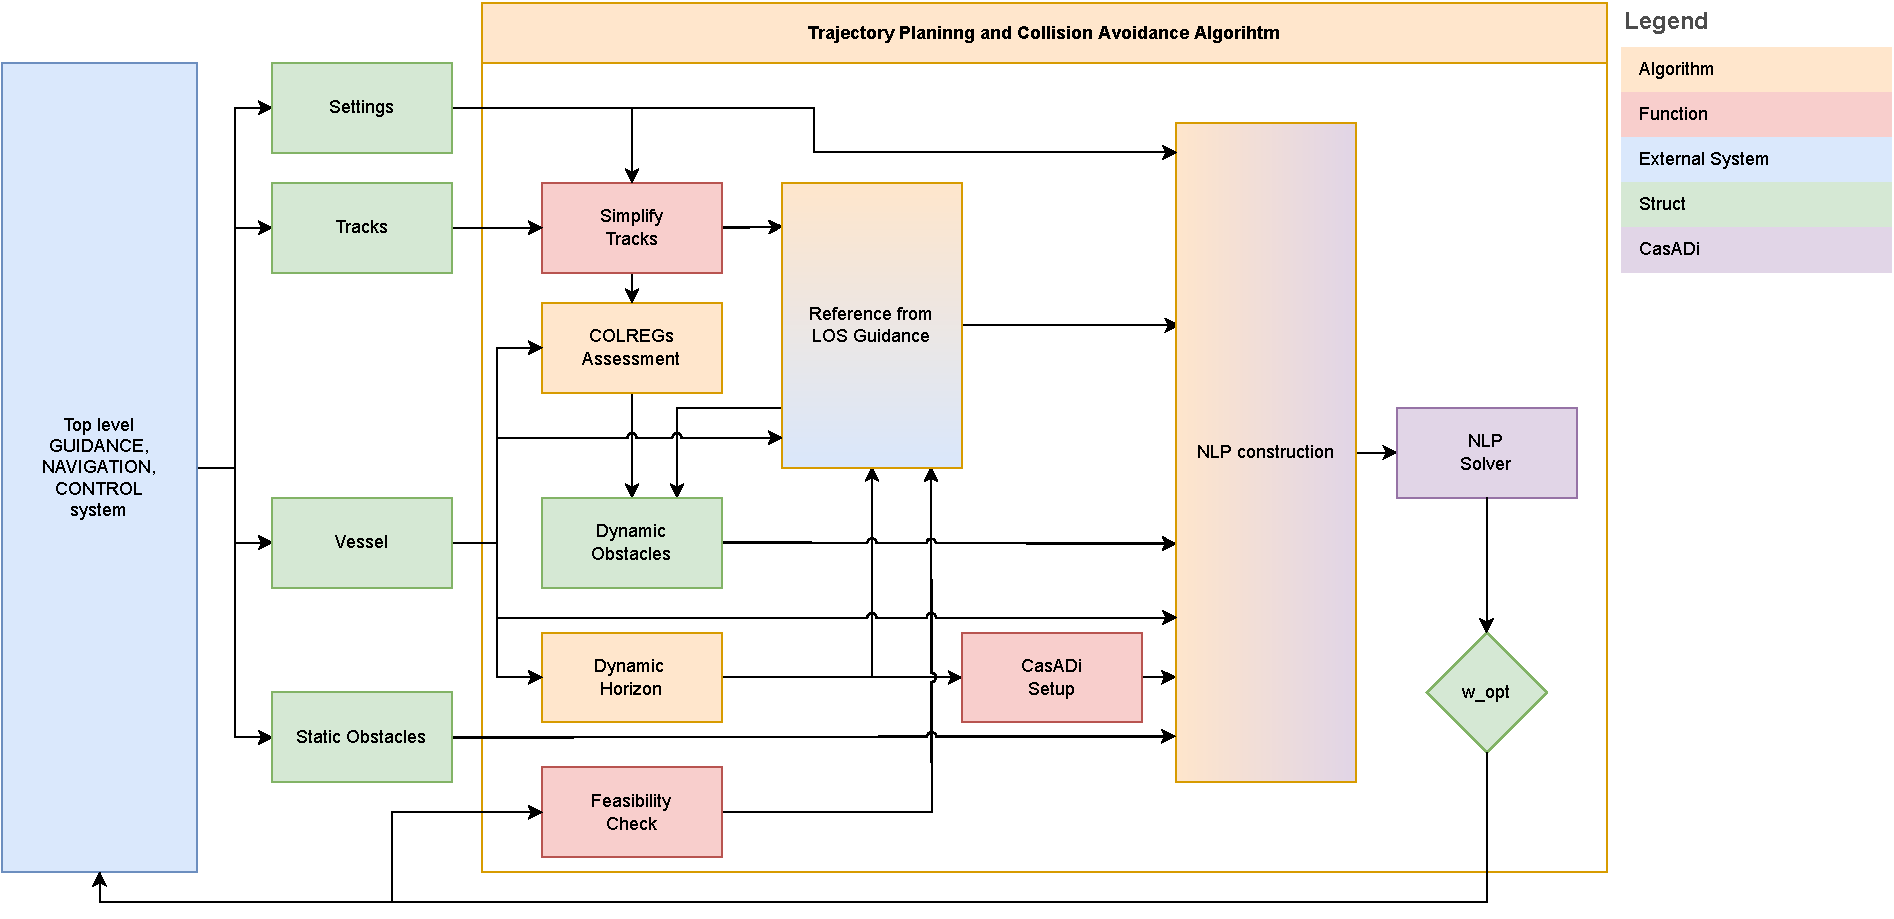
\includegraphics[width=\textwidth]{Images/SimpleSystem.pdf}
    \caption{A simplified overview of the developed algorithm.}
    \label{FIG: Dataflow chart}
\end{figure}
 \newline
This chapter presents a step-by-step walkthrough of the developed trajectory planning and collision avoidance algorithm, and explains some of the
design decisions that were made during development. Additionally, the chapter will include some analysis of problems that arose during development,
and the implementations that were made to overcome them. First the general data flow of the algorithm is presented so that an intuition
can be gained as for how the individual parts of the algorithm are connected. Secondly each step of the algorithm is presented in the order of execution
from top to bottom. Lastly a brief look at how the output from the algorithm is put to use. 

% The author wants to stress that while the trajectory planner is presented as a finished product, the algorithm was in active development until 12 days before
% the thesis deadline. The code will have bugs, there will be unreadable spaghetti code, and at times logical errors. The code should have been delivered
% as an attachment/appendix, or it can be found on GitHub at: (TODO: LINK).
The algorithm was developed in MATLAB and the whole project repo can be found at: \url{https://github.com/ErlHes/TrajectoryPlanning_masteroppgave}

% (TODO: enten i dette kapittelet eller i discussion må det skrives om tallverdi valg på funksjoner som dcpa grense etc.)
% (TODO: bør vel også nevne at koden er skrevet i MATLAB? er ikke det mest brukte kodespråket i verden).

\subsection{Data flow} %(TODO: eller Overview?)
% \begin{itemize}
%     \item Begin by explaining the idea behind how the algorithm should work.
%     \item This chapter will need diagrams.
%     \subitem input $\rightarrow$ ??? $\rightarrow$ output
%     \subitem show how the internal functions parse data
%     \item Serves as a good overview of the whole algorithm.
% \end{itemize}
The core of the design is to construct a path following trajectory that is simultaneously able to comply with \gls{COLREGs} and avoid getting stuck
on terrain or other obstacles. The data flow of the algorithm is depicted in Figure \ref{FIG: Dataflow chart}, 
to avoid clutter the diagram does not include every subfunction and minor detail, it's a
representative diagram, not a blueprint. On the left we begin with a higher level system, the algorithm
relies on getting information about its own vessel and information about other ships, in the diagram called "tracks". Additionally,
static obstacles and miscellaneous other settings for both debugging and behavior tuning is to be supplied from said higher level system.



The algorithm is designed so that full prediction is the assumed standard prediction level. For testing and debugging purposes the tracks
structure can be modified to emulate the form factor of a simple prediction level, in a real implementation the simplification should not be necessary
as the data in the tracks struct should already be in the correct format for either prediction level.
The data in the tracks struct is parsed through a \gls{COLREGs} assessment algorithm to determine if any of the \gls{Ts}s need to be considered
an active dynamic obstacle. If a \gls{Ts} is deemed to be active the \gls{tCPA} and \gls{COLREGs} situation is determined and kept as a flag. The flag
is stored in a persistent variable that the \gls{COLREGs} assessment algorithm checks to avoid overwriting the classification of an active situation.

Next, the information stored in the Vessel struct, the struct dedicated to the \gls{OS}, is used to calculate the desired time horizon for this call's
\gls{MPC}. Horizon distance and discretization step length are then needed by the CasADi setup function to create the \gls{RK4} method that
discretizes the vessel dynamics. On the very first call of the algorithm the feasibility check is skipped, because there is no previous trajectory to parse,
on all subsequent calls of the function the previously calculated optimal trajectory is checked for infeasibility. 
Feasibility, time horizon and discretization step information is then used to generate a reference trajectory for the \gls{OS}, a trajectory is
also generated for all the \gls{Ts} in the tracks struct, which are used to place dynamic constraints later.

The last step of the setup is to initialize the NLP using the \gls{OS}'s initial conditions, which creates the first
six decision variables of $\bm{\omega_0}$ and the first six elements of the constraint function $\textbf{g}(\bm{\omega})$.
Afterwards, the algorithm iterates through all the control intervals, $NP$, from $K = 0:NP-1$, as decided by discretization step length and time horizon, 
constructing the NLP piece by piece in the following order:\newline
(TODO: Denne kan kanskje gjøres om til sånn fin algorithm type)\newline 
First three new decision variables $\bm{\tau_k}$ are made, the appropriate reference states are extracted from the reference trajectory, making sure
that the heading reference doesn't wrap the wrong way about $[0, 2\pi]$. Then the discretized dynamics are used to integrate one control interval
forward using $\bm{\omega_0}$, $\bm{\tau_k}$, and the reference values. Six new decision variables, $\bm{\omega_k+1}$, and their shooting
constraints are made. Lastly dynamic and static obstacles are placed in $\textbf{g}$ and k is incremented by one.

After the \gls{NLP} is constructed the initial guess for $\bm{\omega}$ is replaced by the previous optimal trajectory if it was feasible.
When the \gls{NLP} is solved the time it took is recorded, and if it didn't take too long to solve we save the solution to be used as the previous
optimal trajectory for the next time the algorithm runs. Some plots for debugging can then be made if desired, and the resulting optimal states
for the next control interval returned as the output of the algorithm.


\subsection{Setup}
% \begin{itemize}
%     \item All the stuff before main loop.
%     \item subsubsection for each 'block' as outlined by the dataflow.
% \end{itemize}

% \begin{itemize}
%     \item when the trajectory planner is called we need to run through some calculations before constructing the NLP problem
%     \item These calcualtions are a mix of situation analysis, simulation settings, and CasADi initialization.
%     \item Some of these calculations could be redundant in a complete control and navigation system,
%     where other modules of the system would calculate the same thing.
%     \item It's also important to remember that the value of many parameters are just guesswork, many of the subfunctions
%     would benefit from a more sophesticated design that are tuned based on the situation the vessel finds itself in.
% \end{itemize}
The setup is all the code that is run from when the trajectory planning algorithm is called, up until the construction of the \gls{NLP}.
This is the modular part of the code, where functionality can easily be added or removed without having to refactor
the rest of the algorithm. Anything from new and improved situational awareness models to reference trajectory creation and
COLREGs compliance ideas slot right into the setup. Of course these mentioned systems could just as well exist outside the
trajectory planning algorithm, but for this thesis it's designed as an all-in-one package.

In the current version of the trajectory planning algorithm there are four major and four minor tasks to get through
in the setup. First the major tasks:
\begin{itemize}
    \item Conduct COLREGs assessment.
    \item Calculate dynamic horizon.
    \item Run CasADi initialization.
    \item Generate reference trajectories for \gls{OS} and \gls{Ts}s
\end{itemize}
and the four minor tasks:
\begin{itemize}
    \item Declare and initialize persistent variables.
    \item Initialize dynamic obstacles, and simplify tracks if needed.
    \item Conduct feasibility check on the previous optimal trajectory if it exists.
    % \item Sanitize initial position to make sure there are no problems with the heading.
    \item Fetch static obstacles, this is only a task because of how the MATLAB simulator is set up.
\end{itemize}

\subsubsection*{Persistent Variables} (TODO: vet ikke helt hvorfor jeg går så grundig til verks...)
In MATLAB, persistent variables are stored in memory when a script has terminated, and is loaded back as they were the next
time the script runs. This can be used to create rudimentary state machines, or to check the outcome of the previous iteration for anomalies.
Persistent variables are declared without an initialization, and the method for initializing them without overwriting every time is shown in Algorithm [\ref{ALG: PERSISTENT}].

\begin{algorithm}[ht]
    \caption{Function: Initialize persistent variable} \label{ALG: PERSISTENT}
    \begin{algorithmic}
        \State \textbf{persistent} Var
        \If{isempty(Var)}
            \State Var $\gets$ Initial value
        \EndIf
    \end{algorithmic}
\end{algorithm}

Because persistent variables persist, it is advised to manually clear the script when starting the MATLAB simulator, otherwise
residual persistent variables from unrelated scenario files can cause debugging problems. In the algorithm there are seven
persistent variables. Two are used to store the optimal trajectory between iterations. One to store the discretized function F, so it doesn't have to be
remade every time the algorithm runs. Another for storing COLREGs flag to act as a state machine. One for storing a variable called "firsttime", 
used to execute code only the first time the algorithm is called. One that enables or disables obstacles, 
only left intact as a debugging tool. And the last one to store the previous iterations heading reference, which is used to prevent a
Wrap-to-2-Pi problem. (TODO: SKriv om hva Wrap-to-2-pi problem er for noe).

The reason there are two persistent variables to store the previous optimal trajectory is poor planning:
the original optimal trajectory was dumped if it took too long to solve the NLP. 
But later when I implemented a feasibility check this would cause issues since feasibility and time-to-solve for the NLP are not necessarily linked.
Saving the previous optimal trajectory twice so that one is use for feasibility check, while the other is the initial guess substitution candidate,
was a very quick hack solution that worked well enough that it survived until the final version of the code.


\subsubsection*{Simplify Prediction}
%Avansert TS prediction må skrives om i background.
%Tracks struct må forklares i background.
% This part of the setup is only required in simulations, the aim is to emulate the 'standard' way target ship (TS) prediction is conducted,
% which is to say constant course and velocity [TODO: Citation needed]. The TS trajectory is changed so that the first waypoint is the current position of the
% ship, and the next waypoint is one nautical mile in the direction of the ships heading. Ideally course over ground would be used instead of heading, however
% in the simulator crab angle and sideslip are not accounted for, therefor heading and course are the same angle.
% Excess waypoints stored in the TS struct are also truncated and the current waypoint index is forcefully set to 1 to prevent index out of range type errors.
This part of the setup is only necessary in simulations, the idea is to prepare the tracks struct so that it can be parsed by the COLREGs assessment algorithm
regardless of desired prediction level. Since it is much easier to truncate excess waypoints and 'step down' from full prediction to simple, than the other way around, the algorithm
was developed with full prediction level as the standard. If it's desired to step down to a simple prediction level the tracks simply need to be parsed though algorithm [\ref{ALG: Simplify Tracks}].

% \begin{lstlisting}
%     for i = 1:size(tracks,2)
%         if simple
%             tracks(i).wp(1:2) = [tracks(i).eta(1);tracks(i).eta(2)];
%             tracks(i).wp(3:4) = [tracks(i).eta(1);tracks(i).eta(2)] +...
%                 1852 * [cos(tracks(i).eta(3)) , sin(tracks(i).eta(3))]';
%             tracks(i).wp = [tracks(i).wp(1:2)' tracks(i).wp(3:4)'];
%             tracks(i).current_wp = 1;
%         end
%         [dynamic_obs(i).cflag, dynamic_obs(i).dcpa, dynamic_obs(i).tcpa] = COLREGs_assessment(vessel,tracks(i),cflags(i));
%         cflags(i) = dynamic_obs(i).cflag;
%     end

% \end{lstlisting}
% (TODO: Bedre med algorithm eller MATLAB script insert?)
\begin{algorithm}[ht]
    \caption{Function: Simplify \gls{Ts} prediction} \label{ALG: Simplify Tracks}
    \begin{algorithmic}
        \For{$i = 1:$size(tracks,2)}
            \If{simple}
                \State tracks($i$).wp(1:2) $\gets$ tracks($i$).eta(1:2)
                \State tracks($i$).wp(3:4) $\gets$ tracks($i$).eta(1:2) \\ \hfill + 1 nmi * [cos(tracks($i$).eta(3)) \ , \ sin(tracks($i$).eta(3))]\textsuperscript{T}
                \State tracks($i$).wp = [tracks($i$).wp(1:2)\textsuperscript{T} \ , \ tracks($i$).wp(3:4)\textsuperscript{T}]
                \State tracks($i$).current\_wp $\gets$ 1
            \EndIf
        \EndFor
    \end{algorithmic}
\end{algorithm}



\subsubsection*{COLREGs assessment}
% The COLREGs assessment function solves two problems; figuring out if\/when a TS vessel will be in close enough proximity that evasive maneuvers might be considered,
% and deciding which of the COLREGs rules will apply for the encounter. The design idea is to first find what the distance at closest point (dCPA) of approach with the TS is, and then
% time until cloest point of approach (tCPA) occurs. If both dCPA and tCPA values are under a set threshold we consider the encounter an active event and run the
% COLREGs situation assessment shown by \cite{Thyri2021b}. %COLREGs assessment is also explained in [TODO: fordypningsoppgaven].

% Finding the dCPA and tCPA between two vessels with constant velocity and course is easily done with a formula as shown by(eller in?) \cite{Kufoalor2018}.
%%%%%(TODO: SKRIV OM ALT DETTE, TING BLE FLYTTET HERFRA TIL KAPITTEL 2.3) %%%%%

%However with our wish for more advanced target ship prediction this formula is not sufficient on it's own.
%In order to achieve 'full coverage' of our intended path,
%nd the projected path of the target ship, we must check the dCPA and tCPA starting at each waypoint in the path of both vessels.
% helper function 'getCPAlist' is constructed to get the list of all dCPAs and their respective tCPAs when given two agent structs (AGENT STRUCTS MÅ FORKLARES I BACKGROUND) as inputs.
%o achieve full coverage the getCPAlist function is ran twice so that the perspective of each agent is considered. 

%In terms of code the function for COLREGs assessment uses the helper function getTCPAlist, which in turns uses three more helper functions. The first helper function vesselReadout
%returns the position and velocity in NED given a vessel struct and waypoint index as input. whereisTS gives the same output but takes an agent and time as input arguments instead.
%Lastly the function ClosestApproach takes the output from vesselReadout and whereisTS and applies the equations \eqref{eq:tCPAdCPA}. The dCPA, tCPA and positions are stored and the
%waypoint index is incremented by one, repeat until all waypoints 

% TODO: Ikke ferdig
% to get a list of all dCPA and tCPAs between two agents, as well as the corresponding positions of both
% agents as they are when the euqations \eqref{eq:tCPAdCPA} are used. getCPAlist 

% \begin{algorithm}[t]
%     \caption{getCPAlist. Denne ble jævelig stygg, beholder den for synlighet}\label{alg:getCPAlist}
%     \begin{algorithmic}[1]
%     \Require{$Agent1. Agent2$}\Comment{Agent is a struct that includes path waypoints}
%     \State $dCPAlist \gets []$
%     \State $tCPAlist \gets []$
%     \State $pos\_OS\_list \gets []$
%     \State $pos\_TS\_list \gets []$
%     \State $timer \gets 0$ \Comment{Initialize timer used to calculate position of Agent2}
%     \For{$i \gets Agent1.current\_wp : agent\_wplist\_length - 1$}
%         \State $[pos_{OS}, vel_{OS}] \gets VesselReadout(Agent1, i)$ \Comment{VesselReadout explained in algorithm...}
%         \State $DisttonextWP \gets $Distance to Agent1's next waypoint
%         \State $TimetonextWP \gets DisttonextWP \div$ Agent1's speed over ground
%         \State $[pos_{TS}, vel_{TS}] \gets whereisTS(Agent2, Timer)$ \Comment{whereisTS explained in algorithm...}
%         \State $[dCPA, tCPA] \gets$ Equation for dCPA \& tCPA as shown by...
%         \State $tCPA \gets tCPA + timer$ \Comment{Add travel time to reach current wp}
%         \State $timer \gets timer + TimetonextWP$
%         \State $pos\_OS\_list \gets [pos\_OS\_list, pos_{OS}]$ \Comment{Append all values to respective list.}
%         \State $pos\_TS\_list \gets [pos\_TS\_list, pos_{TS}]$
%         \State $dCPAlist \gets [dCPAlist, dCPA]$ 
%         \State $tCPAlist \gets [tCPAlist, tCPA]$ 
%         \State $i \gets i + 1$
%     \EndFor
%     \State \textbf{return} $pos\_OS\_list, pos\_TS\_list, dCPAlist, tCPAlist$
%     \end{algorithmic}
% \end{algorithm}

% (TODO: synes dette kapittelet er elendig beskrevet, vet ikke om jeg orker skrive det bedre).

The COLREGs assessment algorithm solves two problems, the first is figuring out if a \gls{Ts} vessel will be within close enough proximity that it should be considered
an active COLREGs situation. The second problem is deciding which COLREGs situation such an encounter might be. For two vessels with constant speed and course this is a rather
simple task; first apply the equations \eqref{eq:tCPAdCPA}, and then run a COLREGs assessment function such as one laid out by (\cite{Thyri2021b}). However, if we want
to take advantage of full prediction level a bit more logic is needed to assure full coverage of the intended path. Another functionality needed to ensure COLREGs compliance
is a state machine that holds onto the designated COLREGs situations, the rules state that once a situation has started it persists until both vessels are clear of each other.

The idea for the implementation in this thesis is to extend the \gls{dCPA} and \gls{tCPA} check so that it's conducted for every waypoint in the \gls{OS} and \gls{Ts} reference path.
That way it's possible to know roughly where both vessels should be at the \gls{dCPA} point. The COLREGs assessment
algorithm is therefor split into two parts; the first part is an extended CPA check, the second part is the COLREGs situation assessment. 

A function getCPAlist is created to take two vessel structs as input, one as the assigned \gls{OS}, and the other the \gls{Ts}. The function iterates through all the waypoints
in the \gls{OS} assigned struct and does three things:
\begin{itemize}
    \item Figure out the pose of the \gls{OS} and \gls{Ts}.
    \item Run the CPA check from said pose.
    \item Calculate the time and distance to next \gls{OS} waypoint so that the pose of the \gls{Ts} at that point can be accurately found.
\end{itemize}
Finding the pose of the \gls{OS} is trivial, the first iteration of the function the pose is just the current position and course of the vessel, for all
subsequent waypoints the waypoints themselves are the position and the heading is the direction towards the next waypoint. The last waypoint does not need to be checked
because at that point the \gls{OS} stops moving. While this is a fantastically simple way of integrating forward through the waypoints, the trade-off is less accuracy of the CPA check
when turning. 
Finding the pose of the \gls{Ts} is slightly more involved since there are no waypoints to lean on, the method here is different from for the \gls{OS}.
To begin we know where the \gls{Ts} is when the check is conducted, time and an assumption of constant velocity is then used to calculate the pose.
% (TODO: hvordan vise dette uten å ta med hele kodesnutten?).
% \begin{lstlisting}
%     function [pos_TS, vel_TS] = whereisTS(tracks,wptstimer)
%     pos_TS = tracks.eta(1:2);
%     vel_TS = tracks.eta_dot(1:2);
%     WPlim = size(tracks.wp,2);

%     pos = tracks.eta(1:2);
%     distance = wptstimer * norm(tracks.nu(1:2),2);
%     WPindex = tracks.current_wp;
%     if WPindex < WPlim
%         distancetonextWP = sqrt((tracks.wp(1,WPindex+1) - pos(1))^2 + ((tracks.wp(2,WPindex+1) - pos(2))^2));
%     else
%         distancetonextWP = 0;
%     end
%     while distance > 0
%         if distance > distancetonextWP
%             pos = tracks.wp(1:2,WPindex+1);
%             distance = distance - distancetonextWP;
%             WPindex = WPindex + 1;
%             if WPindex < WPlim
%                 distancetonextWP = sqrt((tracks.wp(1,WPindex+1) - pos(1))^2 + ((tracks.wp(2,WPindex+1) - pos(2))^2));
%             else
%                 distancetonextWP = 0;
%                 pos_TS = pos;
%                 vel_TS = [0,0]';
%                 distance = 0;
%             end
%         else
%             direction = tracks.wp(:,WPindex+1) - pos;
%             travel = distance / distancetonextWP;
%             pos_TS = pos + travel * direction;
%             vel_TS = rotZ(atan2(direction(2),direction(1))) * tracks.nu;
%             vel_TS = vel_TS(1:2);
%             distance = 0;
%         end
%     end
% end    

% \end{lstlisting}
% Here, wptstimer is calculated as the time it would have taken the \gls{OS} to reach the current active waypoint. 
With the pose of both vessels calculated, the next step is to check the CPA, which is the same equation as \eqref{eq:tCPAdCPA}, the values for
\gls{dCPA} and \gls{tCPA}, as well as the pose of both vessels are stored in vectors for later. The \gls{tCPA} value is also added to a timer which is
used to track how much time is passing for the \gls{OS} to reach the checked waypoints.
The full path CPA check is then run with the vessel inputs flipped, so that the \gls{Ts} waypoints are checked, the lowest values of each CPA list
are then compared to select which \gls{dCPA} is truly the shortest distance. If both dCPA and tCPA are under some set threshold a COLREGs classification is set.
(TODO: [...] as described? det er jo referert til tre forskjellige kilder med metoder, tror det skal være greit forstått).

\subsubsection*{Dynamic Horizon}
% \begin{itemize}
%     \item Dynamic horizon is a balancing act between distance to goal, encompassing all active dynamic obstacles, and not looking to far ahead into the future.
%     \item changing the dynamic horizon is really just changing how many control intervals we want the NLP to have.
%     \item As the distance to goal approaches zero we want the number of control intervals to shrink accordingly, otherwise we end up with too many control intervals stationary at the goal, which can cause problems like the cost function becoming unbalanced.
%     \item If there are active dynamic obstacles we need the dynamic horizon to encompass them.
%     \item we don't want the dynamic horizon to be too short during transit (why not?).
% \end{itemize}
The purpose of the dynamic horizon is to shorten the amount of control intervals when the \gls{OS} approaches the final destination. The reason for this
is that having many control intervals stationary at the end position can unbalance the cost function and lead to poor performance for the remainder of the path.
The dynamic horizon can also be coded so that it's dynamic with respects to COLREGs situations; always having enough control intervals to clear the further out
COLREGs situation, but less control intervals than the nominal value so the \gls{NLP} can be solved faster, which would lead to a better reactive performance.

The distance between two waypoints $\textrm{WP}_1 = (N_1, E_1)$,  $\textrm{WP}_0 = (N_0, E_0)$  is calculated by the following equation:
\begin{equation} \label{EQ: Distancebetweenpoints}
    D_{1} = \sqrt{(N_1 - N_0)^2 + (E_1 - E_0)^2}
\end{equation}
which means the distance to goal is the sum of all distances between waypoints:
\begin{equation}
    D_{goal} = \sum_{\textrm{wp} = 1}^{N} D_{wp}
\end{equation}
with $\textrm{WP}_0$ being the position of the \gls{OS} and $\textrm{WP}_N$ being the goal. Assuming a near constant velocity the time to
reach goal is:
\begin{equation}
    T_{goal} = \frac{D_{goal}}{\sqrt{u^2 + v^2}}
\end{equation}
where $u$ and $v$ are the surge and sway speeds of the \gls{OS}. It's not necessary for this check to be 100\% accurate, it is expected that the \gls{OS} will deviate from the
path due to physical constraints and obstacles anyway. To prevent accidentally dividing by zero the surge speed is capped at a lower bound value of $0.001m/s$.
\begin{lstlisting}
if vessel.nu(1) < 0.001
    vessel.nu(1) = 0.001;
end
\end{lstlisting}

Now is where there should have been an implementation for comparing the time to reach goal with the greatest active COLREGs situation tCPA, and picked
one of them as the time horizon. Sadly that functionality ended up being implemented wrongly and therefor left out of the final version of the code
because the tCPA list was not sanitized to only include active COLREGs situations. The correct way of determining time horizon should be:
\begin{algorithm}[h]
    \caption{Dynamic Horizon} \label{ALG: DynamicHorizon}
    \begin{algorithmic}
        \If{Any cflag is set}
            \State \textrm{tempselect} $\gets$ \textrm{min value between $T_{goal}$ and maxseconds}
            \State \textrm{finaltime} $\gets$ \textrm{min value between tempselect and $Active\_tCPA_{max} + 20$}
        \Else
            \State \textrm{finaltime} $\gets$ \textrm{min value between $T_{goal}$ and maxseconds}
        \EndIf
        \State \textrm{h} $\gets$ \textrm{Desired step length}
        \State \textrm{N} $\gets$ \textrm{ceil(finaltime / h)}
    \end{algorithmic}
\end{algorithm}
 \newline
where h and maxseconds are constants for this thesis, N is the number of control intervals. In the current version of the algorithm only the finaltime under the if
sentence condition is hard-coded to return false, due to the aforementioned poor implementation.


\subsubsection*{CasADi setup}
% \begin{itemize}
%     \item sym x = [N, E, psi, u, v, r]
%     \item sym tau as a free variable
%     \item sym xref as reference
%     \item model parameters
%     \item M, C, D matrix
%     \item xdot \= [nu\_dot, eta\_dot]
%     \item Error in the correct reference frame.
%     \item Why is the cost function the way it is.
%     \item runge-kutta method.
%     \item the final function F that CasADi needs.
%     \item Noe av disse greiene blir dekt av Background, forhåpentligvis.
% \end{itemize}
\begin{table}[ht!]
    \begin{center}
        \caption{Estimated model parameters for Milliampere (\cite{pedersen2019optimization}).}
        \label{TAB: Model parameter values}
        \begin{tabular}{c|c|c}
            \hline
            \textbf{Parameter} & \textbf{Value} & \textbf{Unit}\\
            \hline
            m11 & 2131.80 & Kg\\
            m12 & 1.00    & Kg \\
            m13 & 141.02  & Kgm\\
            m21 & -15.87  & Kg\\
            m22 & 2231.89 & Kg\\
            m23 & -1244.35 & Kgm\\
            m31 & -423.76 & Kgm\\
            m32 & -397.64 & Kgm\\
            m33 & 4351.56 & Kgm\textsuperscript{2}\\
        \end{tabular}
    \end{center}
\end{table}

The CasADi setup is where the vessel model and dynamics from (\ref{CHAP: Vessel Modelling}) are implemented, as well as the cost function and \gls{RK4}
method from (\ref{CHAP: NLP}). As the chapter title suggests, everything is implemented using CasADi's framework. The pose and velocity vectors
are combined as one SX.sym vector, while the forces and torque is their own vector. A vector for the references is also created.
\begin{lstlisting}
    % System matrices.
    x = SX.sym('x',6); % x = [N, E, psi, u, v, r]'
    tau = SX.sym('tau',3); % tau = [Fx, Fy, Fn]';
    xref = SX.sym('xref',6); % xref = [Nref, Eref, Psi_ref, Surge_ref, sway_ref, r_ref]'
\end{lstlisting}

% (TODO: Kan skrive inn matrisene på nytt så leser slipper å klikke tilbake til kapittel 2 for å huske hvordan de så ut.)
The vessel mass matrix $\textbf{M}$, \eqref{EQ: Mass}, is created with the following parameter values:

while the values for $\textbf{C}$ are $c13 = -m22*x(5)$, $c23 = m11*x(4)$, $c31 = -c13$, $c32 = -c23$. The dampening matrix $\textbf{D}$ was originally
implemented the way (\cite{pedersen2019optimization}) explains, however turned out to be very computationally expensive for the \gls{IPOPT} solver.
For the sake of brevity, and because full scale tests using the Milliampere ferry fell through due to maintenance, the simplified diagonal matrix \eqref{EQ: Dampening_Simple}
was instead implemented, using some very generous dampening factors:
\begin{equation} \label{EQ: Dampening_method}
    \textbf{D} = \begin{bmatrix}
        200 & 0 & 0\\
        0 & 200 & 0\\
        0 & 0 & 1000
    \end{bmatrix}
\end{equation}

The differential equation for $\bm{\nu}$ is then:
\begin{equation}
    \dot{\bm{\nu}} = \textbf{M}\backslash(\bm{\tau} - (\textbf{C}+\textbf{D})*x(4:6))
\end{equation}
which can then be used to integrate $\bm{\nu}$ forward one step-length with simple Euler integration:
\begin{equation}
    \bm{\nu} = x(4:6) + h\dot{\bm{\nu}}
\end{equation}
The equation for $\dot{\bm{\eta}}$ is the same as \eqref{EQ: eta_dot}, with $\psi$ being $x(3)$.
\begin{equation}
    \dot{\bm{\eta}} = \begin{bmatrix}
        \cos(x(3)) & -\sin(x(3)) & 0\\
        \sin(x(3)) & \cos(x(3)) & 0\\
        0 & 0 & 1 \\
    \end{bmatrix} \bm{\nu}
\end{equation}

With everything set up, the cost function L can be created and defined as a CasADi function as so:
\begin{lstlisting}
    %% Cost function and weights.
    Kp = diag([8*10^-1, 8*10^-1]); % Tuning parameter for positional reference deviation.
    Ku = 6.7*10^2; % Tuning parameter for surge reference deviation.
    Kv = 7.2*10^2; % Tuning parameter for suppressing sway.
    Kfy = 1 * 10^-5;
    % Experimental cost on heading reference:
    K_phi = 6*10^-5;

    R2 = [cos(x(3))    -sin(x(3));...
          sin(x(3))    cos(x(3))];
    Error = R2'*(x(1:2) - xref(1:2));

    L = Error'* Kp * Error + Ku * (x(4)-xref(4))^2...
            + Kv * (x(5)-xref(5))^2 + Kfy * tau(2)^2...
            + K_phi * (ssa(x(3)-xref(3)))^2;
    
    %% Continous time dynamics.
    f = Function('f', {x, tau, xref}, {xdot, L});    
\end{lstlisting}

The parameter values on the weights were chosen by trial and error until the trajectory planning algorithm managed
to track a reference path reasonably well. Cost on deviation from heading reference is actually undesirable, in a real use case
for the algorithm disturbances such as wind, waves and currents would knock the heading about and cause undue increases in cost.
(TODO: as discussed in the theory...) The correct course should naturally be found when velocities are restricted to only
surge, the optimal way to move is in the direction of the goal after all. However, one of the quirks of using numerical optimization 
to guide a vehicle is that the solver has no idea what a boat or a heading is. If the reference trajectory experiences a discontinuous
jump in course by leaving the bounds of $[0, 2\pi]$ and wrapping around the algorithm might have the great idea to turn the long way around.
A miniscule cost associated with turning the wrong way was experimented with to mitigate that possibility.

The last step in the CasADi setup is to discretize the continuous time dynamics by using a \gls{RK4} method:
\begin{lstlisting}
    % Discrete time dynamics.
    M = 4; %RK4 steps per interval
    DT = T/N/M;
    X0 = MX.sym('X0',6);
    Tau = MX.sym('Tau',3);
    Xd = MX.sym('Xd',6);
    X = X0;
    Q = 0;
    for j=1:M
        [k1, k1_q] = f(X, Tau, Xd);
        [k2, k2_q] = f(X + DT/2 * k1, Tau, Xd);
        [k3, k3_q] = f(X + DT/2 * k2, Tau, Xd);
        [k4, k4_q] = f(X + DT * k3, Tau, Xd);
        X=X+DT/6*(k1 +2*k2 +2*k3 +k4);
        Q = Q + DT/6*(k1_q + 2*k2_q + 2*k3_q + k4_q);
    end
    F = Function('F', {X0, Tau, Xd}, {X, Q}, ... 
                    {'x0', 'tau', 'Xd'}, {'xf', 'qf'});
\end{lstlisting}

If you are wondering why the system is initialized with SX.sym but the RK4 method uses MX.sym I have
no answer; CasADi's example pack includes an example for direct multiple shooting, that example includes an RK4 method on the form shown above.
Since my algorithm uses the direct multiple shooting example as a skeleton this RK4 method with MX.sym was carried along until the final version.

Once we have constructed F it can be stored as a persistent variable in MATLAB, then there is no need to rerun CasADi setup potentially saving
milliseconds.

%  If the reference turns from a heading due 10\textdegree
% to a heading due -10\textdegree the algorithm might decide that the best course of action is a 340\textdegree yaw clockwise turn.

\subsubsection*{Feasibility check}
% \begin{itemize}
%     \item The feasibility check came from the wish to read out the status report CasADi prints to the command window.
%     \item It's very important to know if the previous iteration of the trajectory planner function yielded a feasible result or not.
%     \item if the result is not feasible the path forward might be completely blocked, in which case reducing our vessel speed is the best option.
%     \item Very simple check, just checks if every point in the previously calculated optimal trajectory is within 5 meters of each other. This is very lenient and should of course change depending on vessel speed.
% \end{itemize}
% The feasibility arose from the wish to be able to read the status report CasADi prints to the command window. The author never figured out how to do that,
% but after many weeks of not trying very hard to solve the problem the idea finally struck.
Later it will be shown how the previous optimal trajectory can be substituted in for an initial guess to feed the \gls{IPOPT} solver. While
that will be discussed later, the need for a feasibility check arose after frustration with the optimal trajectory getting stuck in an
infeasible state. The first idea to check for feasibility was to somehow read the printout CasADi outputs to the MATLAB command window, 
but to the author's knowledge hat turned out to be impossible. Luckily there is a very easy way to conduct the check manually.

In this context feasibility means the trajectory is physically possible, a jump that covers more distance than the vessel
dynamics allows means the trajectory is infeasible. To check for feasibility simply iterate through each point in the previous
optimal trajectory and check the distance to the next one. Distance is calculated with the same general formula as \eqref{EQ: Distancebetweenpoints}.
If the distance between two points is greater than some set limit then the trajectory is deemed to have been infeasible, which will have
ramifications later. In this thesis the limit for feasibility is a very generous five meters, a lot more than the Milliampere ferry's max speed of
two meters per second can move, but obviously this limit must be tuned to fit the vessel it's controlling.

% (TODO: Jeg kan ta med kodesnutt for hver eneste 'task', da vil leser etter hvert få sett alle de viktigste punktene fra algoritmen.)

\subsubsection*{Reference from LOS}
% \begin{itemize}
%     \item I didn't write this \:)
%     \item The important part is that the time discretization is consistent with the trajectory planner's time step
%     \item You don't need to use LOS for reference.
%     \item Position reference and speed reference need to be consitent with each other.
% \end{itemize} 
The theory behind this chapter was thoroughly discussed in (\ref{CHAP: LOS GUIDANCE}), most of the code for this was also provided by
Emil Thyri, the MATLAB simulator's developer, as it is a necessary for simulating \gls{Ts}s. Therefor this chapter will be brief. The logic implemented
is no different from the discussed theory, one modification that was made specifically for this thesis was functionality for reducing the speed
before creating the reference trajectory. If the feasibility check discussed above deems the previous optimal trajectory to have been infeasible, something
has possibly gone very wrong in the path ahead. The feasibility check says nothing about what went wrong, so in absence of information the best
course of action would be to reduce the vessel's speed until the path ahead clears. 

This reference trajectory does not have to be made using LOS guidance, any guidance law for path or trajectory planning can be applied as long as
it is easily discretized to the same step length as the trajectory planning algorithm uses. One important criteria for picking a reference trajectory 
method is to consider runtime, it would be ill-advised to use an algorithm that takes a very long time to calculate a trajectory.

\subsection{NLP Construction and Solver} 
% \begin{itemize}
%     \item inputs\: vessel, ref\_trajectory, static\_obs, dynamic\_obs, F, settings, h, N, previous\_w\_opt.
%     \item sub funksjoner\:
%     \subitem Dynamic Obs.
%     \subitem Static Obs.
%     \subitem integration step.
%     \item output\: w\_opt
% \end{itemize}

With the setup out of the way it's time to construct and solve the \gls{NLP}. This part of the algorithm
mostly consists of piecing together CasADi's framework and calculating constraints. Construction of the decision variable vector $\bm{\omega}$ and the constraint function
vector $\textbf{g}(\bm{\omega})$ is done piece wise in the following way:
\begin{algorithm}[ht]
    \caption{Construction of CasADi sym vectors and their bounds} \label{ALG: general CasADi sym}
    \begin{algorithmic}
        \State Xk $\gets$ MX.sym(['X\_'num2str(k)] , n) \Comment{where n is the amount of elements in Xk}
        \State $\bm{\omega}$ $\gets$ [$\bm{\omega}$ , \{Xk\}]
        \State $\bm{\omega}_{lb}$ $\gets$ [Xk(1)\textsubscript{lb}, ..., Xk(n)\textsubscript{lb}]
        \State $\bm{\omega}_{ub}$ $\gets$ [Xk(1)\textsubscript{ub}, ..., Xk(n)\textsubscript{ub}]
        \State $\bm{\omega}_0$ $\gets$ [Xk(1)\textsubscript{ref}, ..., Xk(n)\textsubscript{ref}] \Comment{Only applicable for the decision variables}
    \end{algorithmic}
\end{algorithm}

Using the general algorithm, the shooting gap constraints look like this as an example:
\begin{lstlisting}
    g = [g {Xk_end - Xk}];
    lbg(g_counter:g_counter+5) = [0; 0; 0; 0; 0; 0];
    ubg(g_counter:g_counter+5) = [0; 0; 0; 0; 0; 0];
    g_counter = g_counter + 6;
\end{lstlisting}
where Xk\_end is the end of the previous integration step and Xk are the newest decision variables, this will be discussed soon.
Here, the length of the upper and lower bounds are pre-allocated to make the \gls{NLP} slightly more computationally efficient,
it adds up over the course of a long simulation. MATLAB will complain about memory allocation for g, 
but testing showed that it was faster to do it this way than pre-allocating a list. 
% (TODO: skulle ønske jeg tok vare på tallene jeg hadde for dette...)


% \subsubsection{NLP initialization}
% \begin{itemize}
%     \item Initial conditions and end of interval coditions, we need the end of one control interval and the beginning of the next to match.
%     \item Tror dette delkapittelet er litt unødvendig
% \end{itemize}

\subsubsection*{Integration step} \label{CHAP: integration step}
% \begin{itemize}
%     \item Getting the correct reference
%     \item make sure all the indexes are correct!
%     \item put the references in w0, speeds up runtime significantly.
% \end{itemize}
To integrate one control interval forward first create three new decision variables for forces using the general form
shown in algorithm [\ref{ALG: general CasADi sym}]. The upper and lower bounds for these decision variables are the max force and torque
the engine can output. The appropriate velocity and position references are then extracted from the reference trajectory. In the case
for this algorithm the reference trajectory calculates velocities in NED, so they will have to be transformed to BODY in order to be useful.
The position reference is straight forward, but the heading reference needs a bit of work to make sure things don't get messy.

To begin with the reference trajectory does not output heading, but it can easily be found by considering the velocity references, which are in NED.
The direction of the velocity in NED is the desired course. We allow ourselves to use this course as heading reference, even though as discussed in the theory;
that's not an ideal situation.

For the first loop of the \gls{NLP} construction it's important to make sure the heading reference is the same signed angle as the initial position heading.
This is done by checking the difference between heading\_ref - initial\_heading versus wrapTo2Pi(heading\_ref) - initial heading. Whichever resulting angle is the smallest
is the version of the heading reference we want to keep. For every k after 0 The heading reference is kept in the correct sign with the following code:
\begin{lstlisting}
    eta_ref(3) = previous_eta_ref(3)...
                 + ssa(eta_ref(3) - previous_eta_ref(3));
    previous_eta_ref = eta_ref; 
\end{lstlisting}
where ssa() is the shortest signed angle of the difference, and previous\_eta\_ref(3) is the heading reference from the previous control interval.

With the references gathered the discretized time dynamics are used to integrate one control interval forward, with the end states of the integration
saved to use as shooting constraints, and the cost saved in an integrator variable. New decision variables are then made for the next control interval and
new shooting gap constraints are made to ensure consistency between the intervals.

In the end it looks something like this:
\begin{lstlisting}
    Tauk = MX.sym(['Tau_' num2str(k)], 3);
        w = [w {Tauk}];
        lbw(7+k*9:9+k*9)= [-800;  -800;   -800];
        ubw(7+k*9:9+k*9) = [800;   800;    800];
        w0(7+k*9:9+k*9) = [0; 0; 0];
        
        % fetch reference values
        eta_dot_ref = [reference_trajectory_los(3:4,k+1);...
                  (atan2(reference_trajectory_los(4,k+2),reference_trajectory_los(3,k+2)) - ...
                   atan2(reference_trajectory_los(4,k+1),reference_trajectory_los(3,k+1))) / h];
        
        surge_ref = sqrt(eta_dot_ref(1)^2 + eta_dot_ref(2)^2);
        nu_ref = [surge_ref;0;eta_dot_ref(3)];     
        eta_ref = [reference_trajectory_los(1:2,k+1); ...
                    atan2(eta_dot_ref(2),eta_dot_ref(1))]; 

        % We want the reference to start close to initial position.
        if k == 0
            unwrap_diff = abs(eta_ref(3) - initial_pos(3));
            wrap_diff = abs(wrapTo2Pi(eta_ref(3)) - initial_pos(3));

            if unwrap_diff > wrap_diff % check if distance between ref 
                            % and init_pos is greater when unwrapped
                eta_ref(3) = wrapTo2Pi(eta_ref(3));
            end
            previous_eta_ref = eta_ref;
        end
        
        %% Heading control
        if k > 0
            eta_ref(3) = previous_eta_ref(3) + ssa(eta_ref(3) - previous_eta_ref(3));
            previous_eta_ref = eta_ref; 
        end            

        xref_i = [eta_ref; nu_ref];
        
        % Integrate until the end of the interval.
        Fk = F('x0', Xk, 'tau', Tauk, 'Xd', xref_i);
        Xk_end = Fk.xf;
        J = J + Fk.qf;
        
        % New NLP variable for state at the end of interval.
        Xk = MX.sym(['X_' num2str(k+1)], 6);
        w = [w {Xk}];
        lbw(10+k*9:15+k*9) = [-inf; -inf; -inf; -2.3; -2.3; -pi/4];
        ubw(10+k*9:15+k*9) = [inf; inf; inf; 2.3; 2.3; pi/4];
        w0(10+k*9:15+k*9) = [xref_i(1); xref_i(2); xref_i(3); xref_i(4); xref_i(5); xref_i(6)];
        
        % Add constraints.
        g = [g {Xk_end - Xk}];
        lbg(g_counter:g_counter+5) = [0; 0; 0; 0; 0; 0];
        ubg(g_counter:g_counter+5) = [0; 0; 0; 0; 0; 0];
        g_counter = g_counter + 6;
\end{lstlisting}

\subsubsection*{Dynamic Obstacles Constraints}
% \begin{itemize}
%     \item When to place constraints
%     \item Where to place them
%     \item How to place them
% \end{itemize}
\begin{figure}[ht!]
    \centering
    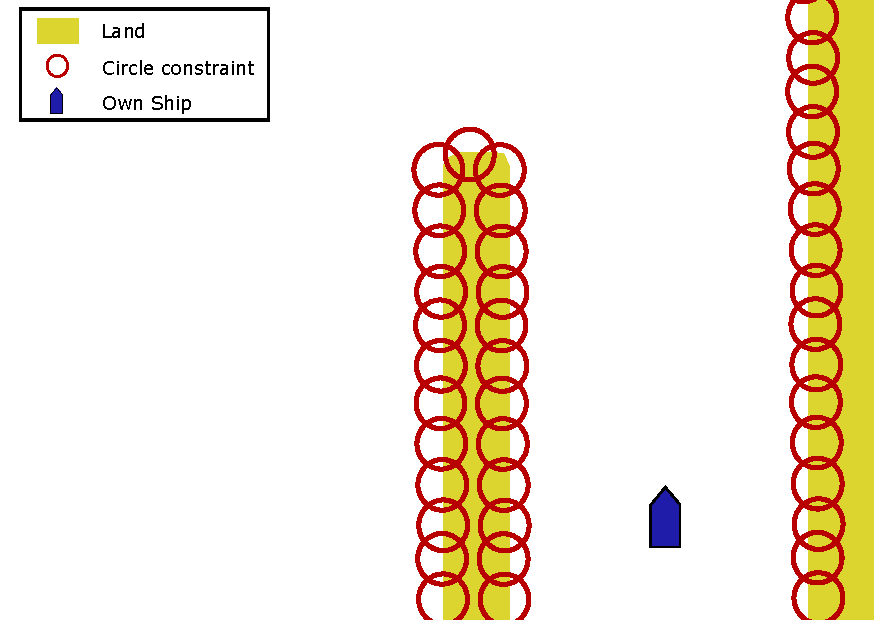
\includegraphics[width=0.66\textwidth]{Images/StaticObs_Naive.pdf}
    \caption{First approach to placing static obstacle constraints, accurate but leads to overload of constraints and poor computational performance.}     \label{FIG: Static Obs Naive approach 1}
\end{figure}
\begin{figure}[ht!]
    \centering 
    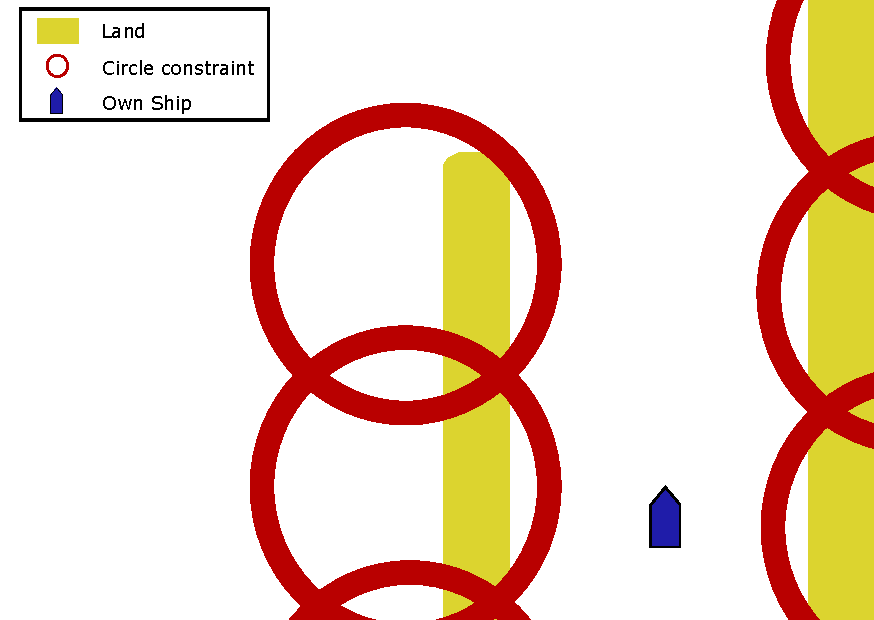
\includegraphics[width=0.66\textwidth]{Images/StaticObs_Naive2.pdf}
    \caption{Second approach to placing static obstacle constraints, avoiding the constraint overload at the cost of greatly reducing available space.}     \label{FIG: Static Obs Naive approach 2}
\end{figure}


The new control interval now needs constraints to ensure a collision free trajectory, starting with the dynamic constraints.
First check if there are any constraints, if there are none the whole step can simply be skipped. Similarly, we want to skip
this step if it's the first time the algorithm is run, the reason why discussed later. (TODO: HUSK DETTE)
Next, iterate through all the \gls{Ts}s in the tracks struct and check their assigned COLREGs flags.
Each COLREGs situation should have their own constraint locations, however the optimal placement
will depend on situation complexity, available space, velocities of the ships involved, and other factors. In
this thesis the placement is simplified greatly by having just pattern for each situation.

The general implementation for placing a constraint is the following function:
\begin{algorithm}[ht]
    \caption{General function for placing dynamic constraint origin point}
    \label{ALG: dynamic constraint origin}
    \begin{algorithmic}
        \State Offsetangle $\gets$ atan2(TS.traj(4,k+1) , TS.traj(3,k+1)) + offset
        \State Offsetdir $\gets$ [ cos(Offsetangle) , sin(Offsetangle) ]
        \State o\textsubscript{dc} $\gets$ TS.traj(1:2 , k+1) + Offsetdist * Offsetdir
    \end{algorithmic}
\end{algorithm}
 \newline
where offset is the angle offset from the \gls{Ts}'s heading, and the Offsetdist is the distance from the center of the
\gls{Ts} to the placement of the constraint origin point. The origin point is placed in $\textbf{g}(\bm{\omega})$
as shown in \eqref{EQ: dynamic constraint in g} while the square of the desired radius of the constraint is placed in
$\textbf{g}(\bm{\omega})_{lb}$.



\subsubsection*{Static Obstacles Constraints} \label{Chap: Method Static Obs}


% \begin{itemize}
%     \item Explain static\_obstacles\_check and the theory for convex-free set
%     \item explain why circles, such as the ones used for dynamic obstacles are insufficient.
%     \item this is sort of similar to finding a cross track error, if that helps to explain what is going on.
% \end{itemize}

% \begin{itemize}
%     \item The first solution for this was to iterate through every polygon in the static obstacle matrix, interpolating
%     every edge to create a saturation of points that would be used as the center for circular constraints, akin to the dynamic
%     obstacles. This was a terrible idea because it meant simulations with lots of static obstacles ended up having hundreds of thounsands
%     of constraints, which made the \gls{NLP} impossible to solve.
%     \item The second solution was to increase the size of the circular constraints significantly so that less were needed. This worked
%     for a while during initial testing and experiments, but eventually proved to obstruct far too much usable space. This was especially
%     noticeable in tighter corridors of water such as a canal or near a pier. Constraints could also end up blocking the waters
%     on the other side of a static obstacle, potentially making it impossible to traverse around oblong static obstacles.
%     \item Explain the trajectory selection, why do we do this? - because the static obstacle function
%     iterates through the selected trajectory to run the scanline intersection algorithm, placing constraints in proximity
%     to the selected trajectory.
%     \item The scanline - polygon intersection function is part of MATLAB's mapping toolbox, creating your own custom intersection
%     check would be really difficult. Polyxpoly outputs the x, y, and edge index for each intersection it finds, some logic is
%     needed to cull duplicates.
%     \item After finding all the intersection points some terrible 2am spaghtti was written to extract only the intersection point
%     and it's corresponding angle, which could have all been done with a lookup table if I were smarter.
%     \item with the intersection point and angle of line the constraint function \eqref{EQ: Static ye}
% \end{itemize}

%% LIMT INN FRA BACKGROUND; BAK INN I TEKSTEN
A singular static obstacle $\mathcal{O}_{s_{i}}$ is presumed to be in the form of a polygon with n corners parameterized
in NED so that:
\begin{equation}
    \mathcal{O}_{s_{i}} = \begin{bmatrix}
                              N_1 & E_1 \\
                              N_2 & E_2 \\
                            \vdots & \vdots\\
                              N_n & E_n
                            \end{bmatrix}^T
\end{equation}
where the point $(N_1 \ , \ E_1)$ is the first point of the polygon defining the obstacle, and the following points are sequential in either a clockwise
or counter-clockwise direction. With N obstacles that can be put together on the form:
\begin{equation}
    \mathcal{O}_s = [\mathcal{O}_{s_{1}} \ , \ \textbf{NaN} \ , \ \mathcal{O}_{s_{2}} \ , \ ... \ , \ \textbf{NaN} \ , \ \mathcal{O}_N] \in \mathbb{R}^{2 \times c}
\end{equation}
where $\textbf{NaN} = [NaN \ , \ NaN]^T$ is inserted between each obstacle to separate them, 
and the column dimension c is dependent on the amount and shape of the obstacles.
%%

Properly incorporating static obstacles into the algorithm proved to be a bit of a hassle. The first solution, seen in 
Figure \ref{FIG: Static Obs Naive approach 1}, was to iterate through every polygon in the static obstacle matrix, interpolating
every edge to create a saturation of points that would be used as the center for circular constraints, akin to the dynamic
obstacles. This was a terrible idea because it meant simulations with lots of static obstacles ended up having hundreds of thousands
of constraints, which made the \gls{NLP} impossible to solve. 
The second solution, seen in Figure \ref{FIG: Static Obs Naive approach 2}, was to increase the size of the circular constraints
significantly so that less were needed. This worked for a while during initial testing and experiments, 
but eventually proved to obstruct far too much usable space. This was especially
noticeable in tighter corridors of water such as a canal or near a pier. Constraints could also end up blocking the waters
on the other side of a static obstacle, potentially making it impossible to traverse around oblong static obstacles.
Eventually the idea of the scan lines came about. At first the scan lines
were going to be used to place circular constraints, but it didn't take long to realize that reusing the logic of cross track
error from LOS guidance would be a much better idea. 

% When the obstacles are gathered in this form, consrtaints can be generated the followig way:\newline
In the final version of the algorithm, static obstacle constraints can be generated the following way:\newline
Consider a fan of scan lines radiating from the \gls{OS} with fixed length and angle. The intersection
point between a scan lines and the line between any two columns in $\mathcal{O}_s$ forms the basis of the constraint 
$\mathbf{o}_{sc} = (o_n \ , \ o_e)$ in NED.\newline
The constraint function is the cross track error between the position of the vessel and a line orthogonal to the scan line which crosses
the point $\mathbf{o}_{sc}$, calculated like in \eqref{EQ: cross and along track error}:
\begin{eqnarray} \label{EQ: Static ye}
    \mathbf{o}_{sc_{ye}} = -\sin(\gamma_p)*(N-o_n) + \cos(\gamma_p)*(E-o_e)
\end{eqnarray}
where (N, E) are the north and east position of the \gls{OS}, and $\gamma_p$ is the angle of the orthogonal line w.r.t NED.
See Figure \ref{FIG: static_obs_ex} for a visualization of the geometry.
The scan lines are generated at each discretized step of the reference trajectory, and every found intersection between a 
line the static obstacles has its own associated cross track error that is added to the function $\textbf{g}(\omega)$:
\begin{equation}
    \textbf{g}(\omega) = \begin{bmatrix}
        \vdots \\
        \mathbf{o}_{sc_{ye}} \\
        \vdots
    \end{bmatrix}
\end{equation}
with the lower bounds of $\textbf{g}(\omega)$ defining the allowed distance between the vessel and the constraint lines, while the upper bounds
should be infinite. This creates a convex free set bound by the static obstacles around the reference trajectory. 
(TODO: kutt den siste setningen hvis jeg ikke kommer på mer å skrive.)

\begin{figure}[th!]
    \centering
    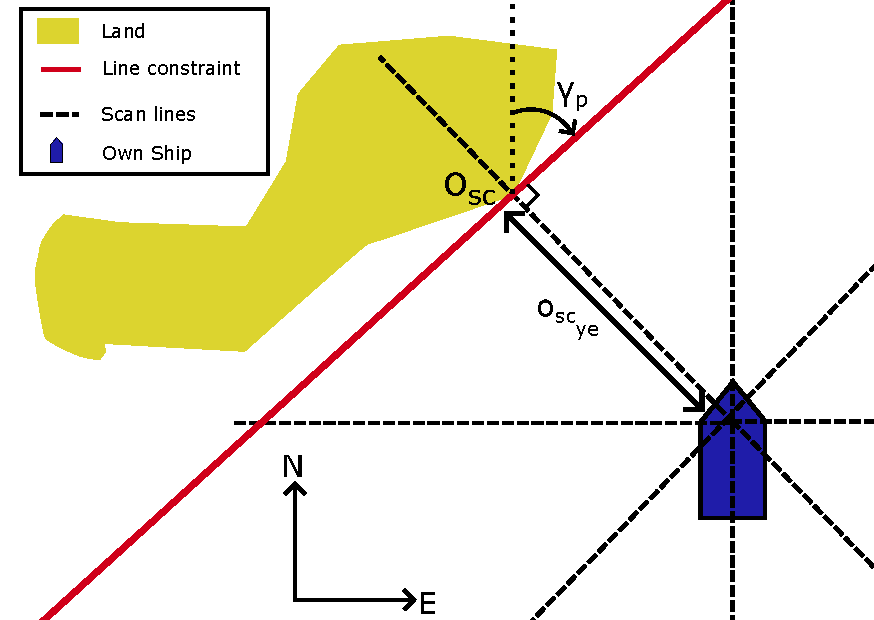
\includegraphics[width=0.7\textwidth]{Images/StaticObs_example.pdf}
    \caption{Geometry for straight line constraints used to handle static obstacles.}
    \label{FIG: static_obs_ex}
\end{figure}

% The current implementation for static obstacles are seen in 
% \ref{FIG: Static Obs Lines} and are computationally very efficient whilst still being very effective at stopping the
% \gls{OS} from colliding with walls. 

\begin{figure}[hb!]
    \centering
    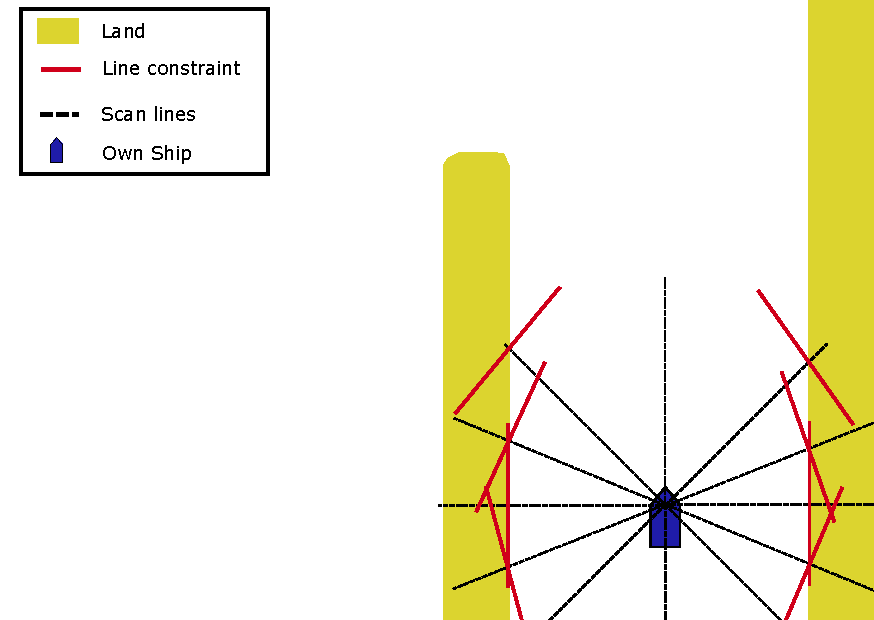
\includegraphics[width=\textwidth]{Images/StaticObs_lines.pdf}
    \caption{Current approach to placing static obstacle constraints, 
    ditching the circular constraints in favor of straight lines based on proximity. 
    Combines the best of both prior versions.}     \label{FIG: Static Obs Lines}
\end{figure} 


The algorithm for creating the intersection points and finding the appropriate angle for the constraint line is a bit involved.
Since every control interval needs its own set of constraints we need to iterate forward in time through decision variables
that don't exist yet. The solution is to instead use the previous optimal trajectory if it exits, or the reference trajectory if we must.
This will create a slight distortion in where the static obstacles end up being placed. But, the distortion is less prominent
the closer we are to the current position of the \gls{OS}, so it's not that big of a deal as the problem corrects itself when it draws near. (TODO: denne distortionen er ikke forklart noe særlig.
det kommer jo av forskjell mellom forrige optimale bane og ny optimal bane kan føre til at statiske hindringer som burde eksistere ikke gjør det eller motsatt.)

While iterating through the selected trajectory the scan lines are fairly easy to construct, but conducting the intersection check is actually very complicated. Luckily
there exists a MATLAB function for just this purpose, polyxpoly, which comes as part of the MATLAB mapping toolbox. Polyxpoly outputs the x, y, 
and an index for which polygon edge were part of the intersection. It does this for every intersection it finds, when we run the check using all the scan lines
and all the static obstacle polygons at the same time this can lead to some duplicate hits. In a similar vein it is possible for a scan line to completely pass through
an obstacle polygon, in which case it would intersect twice, with the second intersection being on the backside of the obstacle. Both the backside intersection and
duplicate intersections are undesirable, the output from polyxpoly can be "sanitized" with the following code snip:
\begin{lstlisting}
    [xi, yi, ii] = polyxpoly(x,y,xbox,ybox);
    % Keep first hit:
    A = [xi, yi, ii];
    [~,uidx] = unique(A(:,3),'stable');
    A_without_dup = A(uidx,:);
    xi = A_without_dup(:,1);
    yi = A_without_dup(:,2);
    ii = A_without_dup(:,3:4);
\end{lstlisting}
The static obstacle constraint parameters can then be collected by combining the xi and yi vectors into a single matrix, keeping in mind that the output
has the x and y-axis opposite from what we have gotten used to by now. The angle of the constraint can then be calculated using some spaghetti code that should
have instead been a lookup table if the author were a bit smarter. The implementation for calculating the angle $\gamma_p$ (here called pi\_p) ended up being:
\begin{lstlisting}
    static_obs_constraints = zeros(3,length(xi));
    for i = 1:length(xi)
        intersectionpoint = [yi(i); xi(i)];
        %horrible 2am spaghetti:
        line = pos - intersectionpoint; % The vector that takes us from intersection point current position
        transposedline = [-line(2);line(1)]; % Get Orthogonal of said vector.
        tangent = intersectionpoint + transposedline; % create point along orthogonal vector
        
        pi_p = atan2(tangent(2) - intersectionpoint(2), tangent(1) - intersectionpoint(1));
        static_obs_constraints(:,i) = [intersectionpoint(1); intersectionpoint(2); pi_p];
    end 
\end{lstlisting}
where pos is the position of the OS. Instead of all this the angle between the intersection point and OS should indicate which scan line resulted
in said intersection, each scan line can only have one orthogonal vector, and they can be pre-calculated and put in a list. You then only have to grab the correct index
from the list to get your angle pi\_p. The constraint function placed in $\textbf{g}(\bm{\omega})$ is Equation \eqref{EQ: Static ye}, with the lower
bound value for g deciding how close the \gls{OS} is allowed the line. In this thesis that lower bound is hard-coded to be 5 meters, but just as with dynamic obstacles
this value should really be some function of the complexity of the situation.



\subsubsection*{Solver}
% \begin{itemize}
%     \item Options, there are many options.
%     \item things to try / were tried for optimizing runtime.
%     \item CasADi really does all the hard work.
% \end{itemize}
After the construction of the \gls{NLP} is finished a solver instance is created with CasADi, selecting \gls{IPOPT}
as the desired solver. Additionally, the solver instance is able to take in a few options for changing tolerances
and tweaking other aspects of the solver. There are three options which are very useful for the algorithm. 
The first is options.ipopt.max\_iter, which lets us set a hardcap on how many iterations the \gls{IPOPT} solver is 
allowed to use. Great for reducing runtime. The second option is the options.ipopt.print\_level, which controls 
how much information is printed to the command window, this has no actual effect solver, 
but printing to command window takes time. Lowering the print level is great for running simulations faster.

In the final version of the algorithm I've set options.ipopt.max\_iter to 200 for the first time 
the algorithm runs, and 400 for the rest. The reason is that the \gls{IPOPT} solver generally gets very close
to a solution in just a few iterations, but then takes a really long time to get all the way to the finish line.
For the first iteration there are no obstacles enabled, if the solver can't get to the optimal solution in 200 iterations
then it's not going to get to one in 2000 either. With obstacles enabled 400 iterations seems like a nice compromise between
wanting a fast solution, and giving the solver enough tries to get reasonably close to an optimum. 

After setting the options and creating the solver instance, the very last task left before solving is to
substitute the initial guess $\bm{\omega}_0$ with the previous optimal trajectory if was deemed feasible
by the feasibility check. Having an initial guess that is close to an optimal solution makes the \gls{NLP}
a lot easier to solve. This is also why the initial guess $\bm{\omega}_0$ is filled with the reference values while
constructing the NLP, it's a lot better to have some initial guess than to guess 0 for everything (\cite{gros2017Lecture}).
Because the amount of control intervals will vary between calls some logic is implemented to make sure the new
$\bm{\omega}_0$ is of the same size. Either by grafting on some reference values or by trimming the end, depending on
if it's too long or short.

The solver instance is then executed and timed, as long as it took less than 30 seconds to solve we save the result for next time
otherwise next iteration will have to rely on the reference as an initial guess.


%  The author wont pretend to know what's the best settings here, recommended
% to leave everything on default except for options.ipopt.max\_iter. 



% \subsection{Alternative Ideas and Lessons}
% Burde kanskje heller gå under discussion, og igjen i future work.
% \begin{itemize}
%     \item Change w0 based on previous solution runtime.
%     \item Gamle versioner av Static\_obs.
%     \item eksperimenter med feasibility check.
%     \item Masse styr med COLREGs assessment, tcpa og dcpa.
%     \item ipopt innstillinger.
% \end{itemize}

\newpage